\documentclass[11pt]{article}
\usepackage{fullpage}
\usepackage{graphicx}
% use Times
% For figures
\usepackage{hyperref}
%set figures fold as figure directory
\graphicspath{ {figures/} }

\usepackage{amsmath}
% For citations
\usepackage{natbib}
\usepackage{tabularx}

\usepackage{subcaption}
% For algorithms and pseudocode
\usepackage{algorithm}

%Adds hyperlinks to your citations automatically
\usepackage{hyperref}
\usepackage{paralist}

% Packages hyperref and algorithmic misbehave sometimes.  We can fix
% this with the following command.
%\newcommand{\theHalgorithm}{\arabic{algorithm}}

\newcommand\tab[1][1cm]{\hspace*{#1}}
\usepackage{float}
%page numbering
\pagenumbering{roman}
\setlength{\textfloatsep}{10pt plus 1.0pt minus 2.0pt}

\title{CS63 Spring 2017 Final Project Report:\\Recognizing Facial Expressions with Machine Learning Algorithms}
\author{Do June Min(dmin1@swarthmore.edu)\\
	Jeremy Han(jhan2@swarthmore.edu)}
%\date{}

\begin{document}
	
	\maketitle
	
	\section{Introduction}
	In this project, we tackled the problem of facial expression recognition
	using machine learning algorithms. Among the algorithms used are support vector machines, decision trees, convolutional neural networks(CNNs), and ensemble methods(Random Forests and AdaBoost). Additionally, we created an ensemble of CNNs(light CNNs) by training a weaker CNN as a binary classifier for each one of the seven emotions, and then aggregating their predictions. As expected, CNNs performed better than other algorithms because they are suited to learn spatial patterns and features. However, we observed that the ensemble of light CNNs fails to deliver a performance on par with the full CNN. In our analysis, we discuss possible reasons behind this. Moreover, different methods of processing and augmenting data are explored. Finally, the performance of each algorithm is evaluated using their accuracy and through a confusion matrix, which we will explain later in this paper. The best performance was achieved by our single CNN, which had an accuracy of 62.8\%.
	
	\section{Method and Details}
	\subsection{Problem and Data set}
	This paper explains the the methods we used to attempt solving the problem of facial expression recognition as formulated by
	\href{https://www.kaggle.com/c/challenges-in-representation-learning-facial-expression-recognition-challenge/data}{Facial Expression Recognition 2013 challenge posted on Kaggle}.
\begin{figure}[!htbp]
  \centering
  \begin{minipage}[b]{0.2\textwidth}
    
\includegraphics[width=\textwidth]{face0}

  \end{minipage}
  \hfill
  \begin{minipage}[b]{0.2\textwidth}
    
\includegraphics[width=\textwidth]{face1}

  \end{minipage}
    \hfill
    \begin{minipage}[b]{0.2\textwidth}
    
\includegraphics[width=\textwidth]{face2}
  \end{minipage}
   \hfill
       \begin{minipage}[b]{0.2\textwidth}
    
\includegraphics[width=\textwidth]{face3}
  \end{minipage}
   \caption{Example images from the data set. Original data vectors were converted and scaled here for better visibility.}
\end{figure}
	
Each example in the data set represents a $48 \times 48$ pixel grayscale image of a face containing one of seven different facial expressions. The seven different facial expressions are anger, disgust, fear, happy, sad, surprise, and neutral. Each example consisted of two columns: emotion and pixels. The pixel column contained a list of numerical values between 0 $-$ 255 representing the pixel values and the emotion column contained a number corresponding to the facial expression in the image.  The data set is comprised of three sections: $28,209$ examples in the training set, $3,589$ examples in the public test set, and another $3,589$ examples in the private test set. The public test set was used to test how well one's classifier worked and the private test set was used to decide the winner of the competition. In this project, we utilized the public test set as a tuning set for various hyper-parameters. After we settled on hyper parameters, we used the private test set to measure the performance of the classifiers. More details about this challenge is described in \cite{goodfellow}.
	
	\subsection{Data Processing and Augmentation}
	Before using the data to train the algorithms, we preprocessed the data. Each original data point is in the form of a vector of size 2304(48 $\times$ 48). While non-convolutional networks accept this form, CNNs require the input to be a 2d image. Thus, we executed a reshaping process so that the original data was converted to a suitable 2d image array.
	
	Moreover, we applied several data processing schemes to make sure that the learning algorithms generalized as much as possible from the data set. The idea of improving a data set using various assumptions and external knowledge about the data is called data augmentation.
	
	\subsubsection{Applying transformations to the data}
	One key idea in data augmentation is that one can increase the size of the data set by applying matrix transformations that preserve the spatial, physical structure of the image data. Unlike general vectors or matrices, images are special in the sense that they encode
	a set of spatially dependent patterns. Thus, certain transformations that preserve this relationship between pixels produce another valid image training example, as it is not identical to the original image, while providing an unseen modified spatial pattern for the algorithm. While there are many such transformations, we focused on and experimented with horizontal flipping(creating a mirror image), slight rotation, and translating the image by some constant.
	
	
	\subsubsection{Adding noise to the training data}
	Another method for augmenting data is adding random noise to images. Similar to the intuition behind dropout technique in training deep neural network, addition of noise aims to make learning algorithms less sensitive to small noises, thereby forcing them to generalize on relevant features and patterns.  Thus, provided with non-noisy data set, the learners would be able to predict in a robust manner. To achieve this, we experimented with randomly choosing several pixels of each image and setting them to random numerical values.
	
	\subsubsection{Applying a predefined image filter to the whole data set}
	Lastly, we tried applying feature-detecting filters to the entire data set, so that the burden of extracting features was lifted from the machine learning algorithms, allowing them to focus more on reasoning with the relevant features to produce better predictions.
	
	%add normal face, sobel filtered face image here
	Sobel filter, an edge detection algorithm often used in image processing, produces an image where the edges are detected and emphasized. This is done by approximating the gradient of the image intensity function. This algorithm is suitable for processing large amounts of image data because its implementation is a simple matrix operation that can be rapidly executed by the GPU. This filter does some of CNN's work by identifying features that make up the image. In this project, we used the implementation from the skimage library \cite{scikit-image}.
	
	%Censure feature detector?
	\subsection{Algorithms}
Since theory and practice suggest that convolutional neural networks are best suited to deal with images, we focused our efforts on CNNs.  We imported the keras library to construct CNNs. However, we also experimented with other learning algorithms to see how they compared to our CNNs.  We imported the sklearn library to implement these algorithms.
			 
	\subsubsection{Support Vector Machine}
	The idea behind SVMs is that transforming data vectors to higher dimensions could help find decision boundaries that might not exist in the original dimensions. Although the computation required to perform this transformation is often costly, a technique called the kernel trick allows for efficient computation of the distance between two vectors in the desired space. Since it is unlikely that a linear mapping would adequately capture the relationship between image vectors and the label, we chose a radial basis function as our kernel because it is theoretically capable of approximating any function. We experimented with various values of $C$, the error term. For larger values of $C$, the SVM will choose a decision boundary with small margin, and with small values of $C$, a hyperplane of larger margin is preferred, even if it results in some misclassifications. We settled with $C=10.0$
	
	\subsubsection{Decision Tree}
	We used the scikit implementation of a decision tree as one of our classifiers. Although it does not make much sense to treat the image as a numerical vector and treat each pixel value as a fixed feature, we included this classifier to compare with the two ensemble methods that use decision trees as their base classifiers: Random Forest and AdaBoost. We used the default parameters for decision trees.
	
	\subsubsection{Random Forest}
	Random Forest is an ensemble method that utilizes bootstrap aggregating(bagging) of the data to create many decision trees. Although each tree might be overfitted to the bootstrapped data on which it is trained, one could reduce overfitting by combining their prediction into one. After experimenting, we fixed the number of base classifiers to 200.
	
	\subsubsection{AdaBoost}
	AdaBoost, or adaptive boosting, combines the advantages of the boosting method and adaptively weighing misclassified examples to produce a learner with high accuracy and low overfitting. After experimenting, we fixed the number of base classifiers to 200.
	
	\subsubsection{Single Convolutional Neural Network}

	 We developed several different CNNs, building them layer by layer. We used the dense layer, which is a fully connected neural network hidden layer where each input node is connected to every output node. This layer provides shared weights. We can also apply an activation to the layer where we specify the type of function of the node, such as relu and sigmoid. 
	
	 We also used a layer called maxpooling2D. In this layer, we reduce the dimensionality of the input using a sliding window that outputs the maximum value it sees. This is done to reduce the number of features and computational complexity of the task, essentially producing a summary of the image. The layer called conv2D is similar to maxpooling2D in that a sliding window is also being used. However, the conv2D is the standard convolution layer that learns deep features about the image.
	
     Additionally, CNNs can support ensemble learning because of dropout layers. An ensemble of CNNs would take too long to properly train for deep learning, so dropout layers allow us to train just one CNN. Dropout layers are layers with nodes that have a probability $p$ of dropping out, a parameter that we can decide. Each time a new example is presented to the CNN, nodes are randomly picked to drop out. This means that the incoming and outgoing weights of the dropped out nodes do not get updated, so it is as if a new architecture was used to learn the example. Consequently, it's as if an ensemble of different architectures are learning the data set, but it is really just one, saving time. When classifying the test set, no nodes are dropped out to receive the benefit of learning from all the different architectures that were created. A link to an image describing the full architecture of the network is included in the appendix.
      
     The following table lists the parameters chosen to train the network.
     
    \begin{table}[!htbp]
\centering
\caption{Training Parameters for Single CNN}
\label{my-label0}
\begin{tabular}{|c|c|}
\hline
Parameter     & Value \\ \hline
Optimizer       &  Stochastic Gradient Descent     \\ \hline
Learning rate &   0.01    \\ \hline
Decay rate    &  $1e-6$     \\ \hline
Momentum      &   0.9    \\ \hline
Loss Function &  categorical cross entropy     \\ \hline
Batch Size    &  128     \\ \hline
Epochs        &  30     \\ \hline
\end{tabular}
\end{table}
To optimize the algorithm, we chose standard Stochastic Gradient Descent with a learning rate of $0.01$. We also set a non-zero decay rate, so that the weights can slowly converge into an optimal configuration. Also, we chose a momentum value of 0.9. Momentum can be understood as an extra parameter that guides the weight space search out of local minima by adding a fraction of the previous weight update to the current one. In practice, updating weights with momentum generally works better than vanilla update. The loss function, which was used to calculate the error of the calculator that was propagated back to calibrate the weights, was categorical cross entropy, which is generally considered to be better than mean square error for classification tasks. The epoch was set to 30 because we observed a sign of overfitting for values higher(training accuracy much higher than validation accuracy and final accuracy not improving after $>30$ epochs.)

	\subsubsection{Group of CNN Binary Classifiers}
The motivation behind constructing a group of binary CNNs is similar to that behind any ensemble method. Instead of having a monolithic, large classifier with many parameters, one could train multiple ``panels of experts" and aggregate their predictions into a single prediction. To achieve this, we created seven CNNs that are limited in layer depth and parameter numbers. Then, we trained each of them on a modified data set that was labeled either 1 or 0, indicating whether the image's label is of the emotion on which the classifier is being trained. In this way, we were able to train a binary classifier for each class of emotions. Then, we output a final prediction by taking the label whose binary classifier had the highest output, meaning that it had the highest confidence in believing the data to belong to a class. The full architecture of each binary network can be accessed through a link in appendix.
    
To train the network, we used the same parameters as a single CNN, with the exception of the loss function and epoch. We replaced categorical cross entropy with binary cross entropy, since each light CNN is a binary classifier for a single emotion label. Also, because training 7 networks was very time-consuming and each binary classifier reached a fairly high accuracy($-$90\%) within few epochs, we set the epoch $=3$.
    
	\subsection{Evaluation Methodology}
	To evaluate the result of the classifiers, we used accuracy to measure the performance. We also utilized confusion matrices to identify and visualize with which category a certain classifier was most having trouble. A confusion matrix is basically a breakdown of the testing examples by its predicted label and its ground truth. Although the matrix itself does not provide a single metric denoting a classifier's performance, one can easily identify the strength and weak spots of a classifier by inspecting it. Also, to make sure that the outcome was not heavily influenced by noise, we conducted 10 iterations of testing for each classifier and averaged the accuracy.
	
	Moreover, we reduced the possibility that our classifiers were overfitted to the training set by setting aside a set to be used as a tuning set for hyper-parameters. For better generalization, we could have merged the public test set to the training set. However, this resulted in overfitting, as we would be "training"(picking hyper-parameters so that the accuracy is increased) our algorithm with our test set. This mistake of using one's training set to pick/train the model is called the cardinal sin of machine learning.
	
	\section{Results}
	
	\subsection{Experiment Results}
	With several experiments, it became evident that data processing methods other than horizontal flipping were irrelevant in providing more information to the algorithms. Even more, they were causing algorithms to overfit, since those transformations were either creating images too similar to the original, which led to overfitting, or destroying the spatial structure of the image(noise). Thus, to save computational resources and time, we conducted our final evaluation with data processed only by horizontal flipping, doubling the data.	
	
	The following table lists the average accuracy of each classifier in the final experiment. The single CNN performed the best; the group of light CNNs followed with a wide margin of 10.2\%.
	
	
	\begin{table}[!htbp]
\centering
\caption{Accuracies of each classifier, average from 10 iterations of testing}
\label{my-label2}
\begin{tabular}{|c|c|}
\hline
Classifier             & Accuracy \\ \hline
Support Vector Machine &    41.0\%      \\ \hline
Decision Tree          &   34.8\%       \\ \hline
Random Forest          &  46.2\%        \\ \hline
AdaBoost               & 48.4\%          \\ \hline
Single CNN             &  \textbf{62.8\%}         \\ \hline
Group CNN              &  52.6\%        \\ \hline
\end{tabular}
\end{table}

Although accuracy is arguably the most important metric for evaluating a multiclass classifier, it is useful to consider different ways of analyzing the result. To this end, we generated a confusion matrix for each classifier. The following matrices are obtained after testing each algorithm once.

\begin{figure}[!htbp]
  \centering
  \begin{minipage}[b]{0.48\textwidth}
    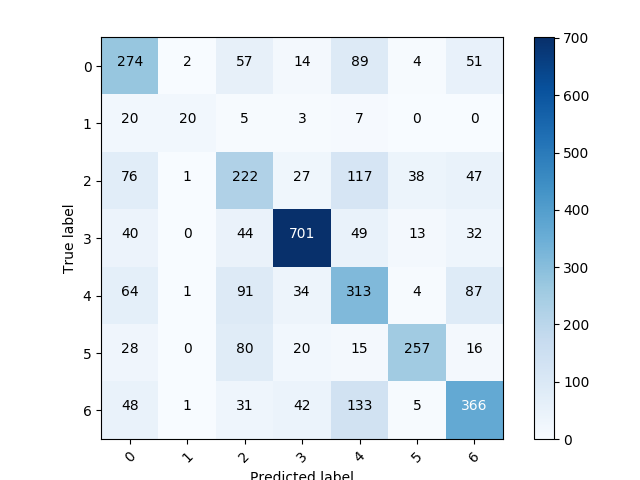
\includegraphics[width=\textwidth]{confusion_conv}

  \end{minipage}
  \hfill
  \begin{minipage}[b]{0.48\textwidth}
    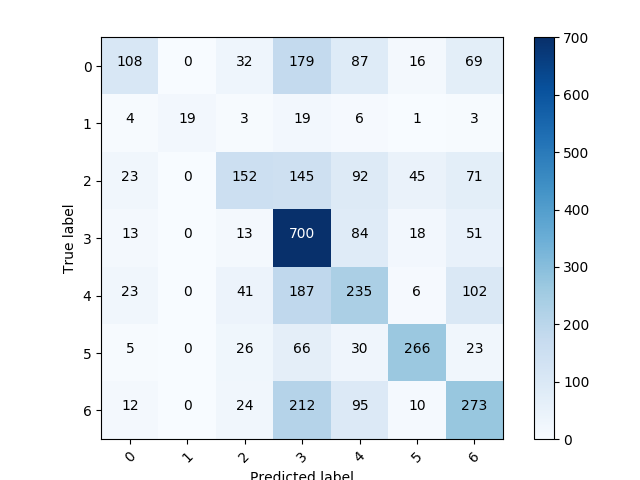
\includegraphics[width=\textwidth]{confusion_ada}

  \end{minipage}
    \hfill
   \caption{Example confusion matrices of Single CNN(left) and AdaBoost(right)}
\end{figure}

Note that both algorithms were able to correctly identify most ``happy''(3) faces. On the other hand, neither of them had much success in distinguishing ``disgust''(1) from other emotions. There is also a subtle difference in this conclusion. Note that the Single CNN most frequently confused between ``anger'' and ``disgust''(20 and 20), while AdaBoost mixed between ``happy'' and ``disgust''(19 and 19). While the former is an error often made by humans, confusion of the latter sort rarely happens. This suggests that the Single CNN is making decisions based on learned features of the images.

	\subsection{Analysis of Result}
While we expected variations of CNNs to outperform other algorithms, the result suggests that the single, strong CNN fares better than an ensemble of weak CNNs. We attribute the relative failure of the ensemble method to its construction.

In ensemble methods, it is crucial that each base learner is i) better than random guessing, and ii) is uncorrelated to others. While our construction satisfies the first condition, it is very likely that 
each binary classifier is correlated, since they share a uniform architecture and training set. This is a design flaw that can be mitigated by randomly selecting a subset of the data for training or differing the architecture of each network.

Moreover, there are other theoretical limitations to an ensemble of neural networks. First, no matter how compact a neural network is compared to other networks, it is still deep in the sense that it utilizes multiple layers of nodes to learn representations of data. This goes directly against the idea of using multiple weak learners. It is also problematic how to properly aggregate the outputs of the weak learners. Merely taking the label with highest probability abandons information gained through deep network. If we try to avoid this by connecting the outputs(a vector of size 7), then it would be a very inefficient network in which relevant representations of the data are ignored in the final layer. Thus, we conclude that directly applying the idea behind ensemble method to CNN does not provide any advantage over using a normal deep CNN. 

%Class Imbalance
	
	\section{Conclusions}
	Comparing the result of our experiment with systems submitted to the finished Kaggle challenge, we see that our best learner, Single CNN, trails the top performer(username RBM, with 71.162\% accuracy) by about 10 percent. Although our system would have ranked on Top 10, it should be noted that this challenge was hosted 4 years ago. Thus, it is expected that state-of-the-art systems with new techniques and learning models could vastly outperform any of the reported scores.
	
	Moreover, many practical image classification systems do not train their network from scratch. In fact, many utilize a pre-trained large scale image classification network, such as AlexNet\cite{NIPS2012_4824} or VGG16\cite{1409.1556}. These systems load up the pretrained weights of a large network and connect its output to a custom designed layer. By freezing the pretrained network and finetuning the custom top layer, the systems exploit the hierarchical representations of the image learned from a much larger data set(ImageNet\cite{imagenet_cvpr09} contains over ten million hand-annotated images) to solve a simpler problem.  
	
	However, this project demonstrates that even with a relatively simple network architecture and a simple data augmentation scheme, it is possible to achieve a reasonably high performance with a CNN trained from scratch. Although we have failed to increase our accuracy beyond 62\% using this method alone, we believe that the possibility of improving the system by leveraging deeper representation encoded in large, pretrained systems provides an interesting direction for future research.
	
	\section*{Appendix}
	(1) \href{https://github.swarthmore.edu/cs63-s17/lab10-dmin1-jhan2/blob/master/paper/figures/conv2_model.png}{Link to Single Convolutional Network Architecture}\\
	\noindent\\
	(2) \href{https://github.swarthmore.edu/cs63-s17/lab10-dmin1-jhan2/blob/master/paper/figures/light_conv_model.png}{Link to Light Convolutional Network Architecture}\\
	\noindent\\
	(3) \href{https://www.kaggle.com/c/challenges-in-representation-learning-facial-expression-recognition-challenge/data}{Link to Facial Expression Recognition 2013 challenge posted on Kaggle}
	
	\bibliographystyle{unsrt}
	\bibliography{references}
	
\end{document}
	The layers of CNN serve to convolute the image, which in this case means to take a sliding window over different regions of the image. The different regions of the image are connected through shared weights. The significance of this is that the CNN learns to detect specific features in the image because of the interconnections of the shared weights. 
	

		 
		 
		
